\documentclass{article}
\usepackage[utf8]{inputenc}
\usepackage{amsmath}
\usepackage{float}
\usepackage{fullpage}
\usepackage{parskip}
\usepackage{graphicx}

\title{Ph20 Assignment 1}
\author{Ung Shu Fay}

\begin{document}
\maketitle

\section{Lissajous Figures}
	\begin{align}
		X(t) &= A_x \cos (2 \pi f_x t) \\
		Y(t) &= A_y \sin(2 \pi f_y t + \phi) \\
		Z(t) &= X(t) + Y(t)
	\end{align}

	If $f_x/f_y$ is a rational number, the graph of $X(t)$ against $Y(t)$ is a closed curve.

	\begin{figure}[H]
		\centering
		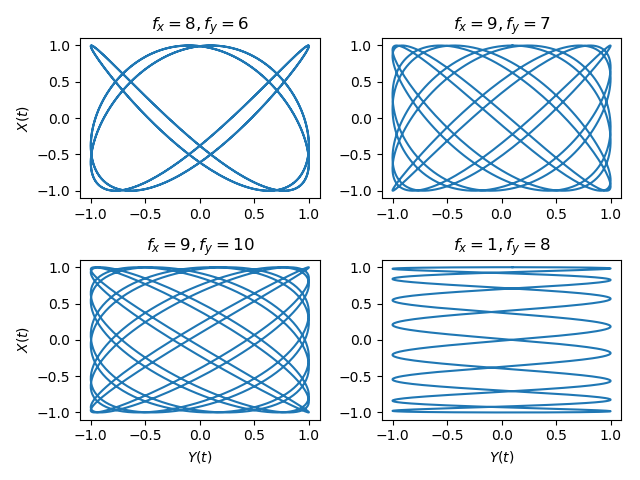
\includegraphics[scale=0.6]{plots/rational.png}
		\caption
		{
			Plots of $X(t)$ against $Y(t)$ for rational $f_x/f_y$. The values of $f_x$ and $f_y$ were selected randomly. Graphs were generated with $A_x = A_y = 1$, $\phi = 0.1$, $\Delta{t} = 0.001$ and $N = 1000$.
		}
	\end{figure}

	\subsection{$f_x/f_y$ and the Shape of the Curve}
		For $f_x/f_y < 1$, as the ratio increases, the number of points where the curve intersects itself increase.

		\begin{figure}[H]
			\centering
			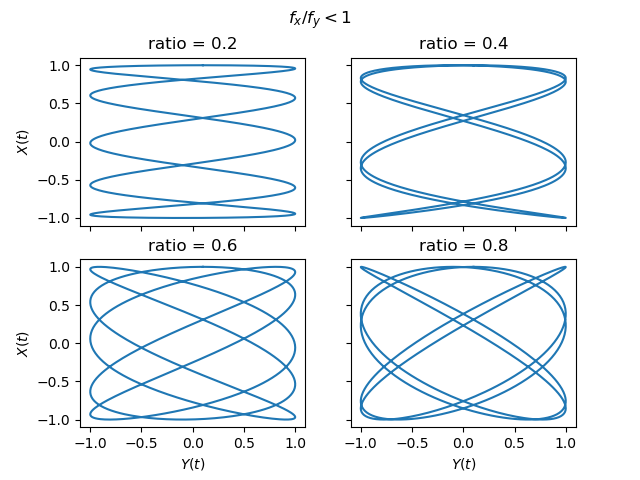
\includegraphics[scale=0.7]{plots/ratio1.png}
			\caption
			{
				Plots of $X(t)$ against $Y(t)$ for $f_x/f_y < 1$. Graphs were generated with $f_y = 5$, $A_x = A_y = 1$, $\phi = 0.1$, $\Delta{t} = 0.001$ and $N = 1000$ for $f_x/f_y = 0.2, 0.4, 0.6, 0.8$.  
			}
		\end{figure}

		For $f_x/f_y > 1$, the curves resemble overlapping sinusoids with the endpoints connected together. As the ratio increases, the number of peaks and the number of points of intersection increase.

		\begin{figure}[H]
			\centering 
			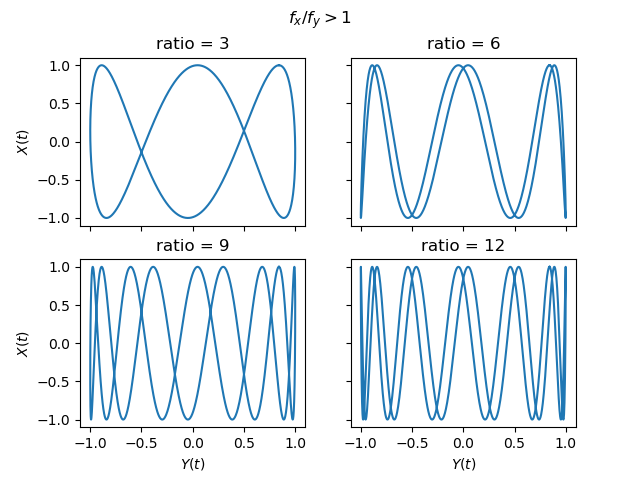
\includegraphics[scale=0.7]{plots/ratio2.png}
			\caption
			{
				Plots of $X(t)$ against $Y(t)$ for $f_x/f_y > 1$. Graphs were generated with $f_y = 5$, $A_x = A_y = 1$, $\phi = 1$, $\Delta{t} = 0.0001$ and $N = 2000$ for $f_x/f_y =$ 3, 6, 9, 12.  
			}
		\end{figure}

	\subsection{$\phi$ and the Shape of the Curve}
		Setting $f_x=f_y$, the shape of the curve was observed while the phase $\phi$ was varied. The plots trace out ellipses for $n \neq k/2$ where $k$ is odd, and straight lines when $n = k/2$. This is due to the fact that the graphs of $\mathrm{sin}$ and $\mathrm{cos}$ are shifted by a phase of $\pi/2$. 

		\begin{figure}[H]
			\centering
			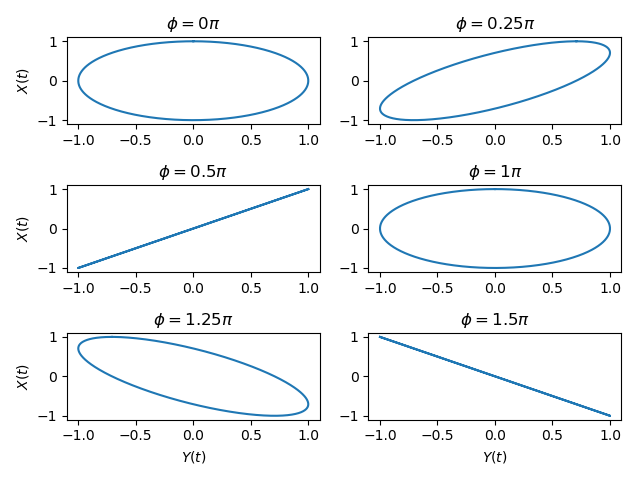
\includegraphics[scale=0.7]{plots/phase.png}
			\caption
			{
				Plots of $X(t)$ against $Y(t)$ for different values of phase $\phi$. Graphs were generated with $f_x = f_y = 1$, $A_x =A_y = 1$, $\phi = 1$, $\Delta{t} = 0.001$ and $N = 1000$ for $\phi = n \pi$ where $n = 0, \ \frac{1}{4}, \ \frac{1}{2}, \ 1, \ \frac{5}{4}, \ \frac{3}{2}$.  
			}    
		\end{figure}

		In electronic circuits, if two alternative currents are out of phase by $\phi$, plotting the currents against each other and adjusting them until a horizontal ellipse is seen on the oscilloscope means they are in phase or in antiphase with each other. 

\section{Beats}
		\begin{figure}[H]
			\centering
			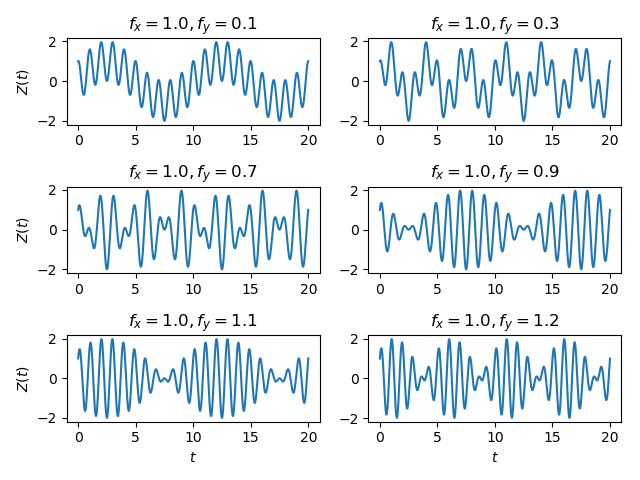
\includegraphics[scale=0.7]{plots/beats.png}
			\caption
			{
				Plots of $Z(t)$ against $t$. Beats produced by setting similar values for $f_x$ and $f_y$. Graphs were generated with $A_x = A_y = 1$, $\phi = 0$, $\Delta{t} = 0.01$ and $N = 2000$ for $f_x = 1$ and $f_y =$ 0.1, 0.3, 0.7, 0.9, 1.1, 1.2.     
			}
		\end{figure}

\section{Thoughts}
	The programming was rather fun to do, especially in investigating the properties of the graphs. The assignments were not too difficult.
	
	I havn't really programmed in other languages other than Python, but taking CS2 this term in C++ made me appreciate the simplicity and level of abstraction Python provides for the user. I do agree with Guido Van Rossum - Python is incredibly powerful and is pleasurable work with (no segmentation faults!).

\end{document}
